\documentclass{beamer}

\usepackage[utf8]{inputenc}
\usepackage[brazil]{babel}

\usepackage{verbatim}

\usepackage{graphicx}

\usepackage{listings}
\usepackage{color}

\definecolor{mygreen}{rgb}{0,0.6,0}
\definecolor{mygray}{rgb}{0.5,0.5,0.5}
\definecolor{mymauve}{rgb}{0.58,0,0.82}
\definecolor{mybckg}{rgb}{0.95,0.95,0.95}
\lstset{
  backgroundcolor=\color{mybckg},  % choose the background color; you must add \usepackage{color} or \usepackage{xcolor}
  basicstyle=\footnotesize,       % the size of the fonts that are used for the code
  breakatwhitespace=false,         % sets if automatic breaks should only happen at whitespace
  breaklines=true,                 % sets automatic line breaking
  %captionpos=b,                    % sets the caption-position to bottom
  %commentstyle=\color{mygreen},    % comment style
  deletekeywords={...},            % if you want to delete keywords from the given language
  escapeinside={\%*}{*)},          % if you want to add LaTeX within your code
  extendedchars=true,              % lets you use non-ASCII characters; for 8-bits encodings only, does not work with UTF-8
  frame=single,                    % adds a frame around the code
  keepspaces=true,                 % keeps spaces in text, useful for keeping indentation of code (possibly needs columns=flexible)
  columns=flexible,
  %keywordstyle=\color{blue},       % keyword style
  %language=bash,                   % the language of the code
  morekeywords={*,...,Hello,LS,Update},            % if you want to add more keywords to the set
  %numbers=left,                    % where to put the line-numbers; possible values are (none, left, right)
  %numbersep=5pt,                   % how far the line-numbers are from the code
  %numberstyle=\tiny\color{mygray}, % the style that is used for the line-numbers
  rulecolor=\color{black},         % if not set, the frame-color may be changed on line-breaks within not-black text (e.g. comments (green here))
  %showspaces=false,                % show spaces everywhere adding particular underscores; it overrides 'showstringspaces'
  %showstringspaces=false,          % underline spaces within strings only
  %showtabs=false,                  % show tabs within strings adding particular underscores
  %stepnumber=2,                    % the step between two line-numbers. If it's 1, each line will be numbered
  %stringstyle=\color{mymauve},     % string literal style
  tabsize=2,                       % sets default tabsize to 2 spaces
  %title=\lstname                   % show the filename of files included with \lstinputlisting; also try caption instead of title
  literate=
  {á}{{\'a}}1 {é}{{\'e}}1 {í}{{\'i}}1 {ó}{{\'o}}1 {ú}{{\'u}}1
  {Á}{{\'A}}1 {É}{{\'E}}1 {Í}{{\'I}}1 {Ó}{{\'O}}1 {Ú}{{\'U}}1
  {à}{{\`a}}1 {è}{{\'e}}1 {ì}{{\`i}}1 {ò}{{\`o}}1 {ù}{{\`u}}1
  {À}{{\`A}}1 {È}{{\'E}}1 {Ì}{{\`I}}1 {Ò}{{\`O}}1 {Ù}{{\`U}}1
  {ä}{{\"a}}1 {ë}{{\"e}}1 {ï}{{\"i}}1 {ö}{{\"o}}1 {ü}{{\"u}}1
  {Ä}{{\"A}}1 {Ë}{{\"E}}1 {Ï}{{\"I}}1 {Ö}{{\"O}}1 {Ü}{{\"U}}1
  {â}{{\^a}}1 {ê}{{\^e}}1 {î}{{\^i}}1 {ô}{{\^o}}1 {û}{{\^u}}1
  {Â}{{\^A}}1 {Ê}{{\^E}}1 {Î}{{\^I}}1 {Ô}{{\^O}}1 {Û}{{\^U}}1
  {œ}{{\oe}}1 {Œ}{{\OE}}1 {æ}{{\ae}}1 {Æ}{{\AE}}1 {ß}{{\ss}}1
  {ç}{{\c c}}1 {Ç}{{\c C}}1 {ø}{{\o}}1 {å}{{\r a}}1 {Å}{{\r A}}1
  {€}{{\EUR}}1 {£}{{\pounds}}1,
  %basicstyle=\ttfamily
}

\useoutertheme{infolines} % add a footline 
\usetheme{Frankfurt}
%\setbeamertemplate{items}[square] % changes the markers, ball: 3-dimensional balls, circle: 2-dimensional (flat) circles, rectangle: rectangles, default: triangles 
%\setbeamertemplate{section in toc}[circle]
\setbeamertemplate{section in toc}[ball unnumbered]
\setbeamertemplate{enumerate item}[square]
\setbeamertemplate{itemize item}[triangle]
\setbeamertemplate{itemize subitem}[circle]
\setbeamertemplate{blocks}[rounded][shadow=true] % add rounded corners and a shadow to the box that surrounds the theorem
\setbeamertemplate{navigation symbols}{} % disable the drawing of navigation icons

\newlength{\wideitemsep}
\setlength{\wideitemsep}{\itemsep}
\addtolength{\wideitemsep}{10pt}
\let\olditem\item
\renewcommand{\item}{\setlength{\itemsep}{\wideitemsep}\olditem}

\title[Localização para Robôs Móveis]{Localização \textit{indoor} para robôs móveis}
\author[Edileuton H. de Oliveira]{Edileuton Henrique de Oliveira}
\institute[UFPR]{
  Departamento de Informática\\
  Universidade Federal do Paraná\\
  Bacharelado em Ciência da Computação\\
  Trabalho de Graduação\\
  Orientador: Prof. Eduardo Todt.
}

\usepackage{remreset}
\makeatletter
\@removefromreset{subsection}{section}
\makeatother


\begin{document}
%\maketitle

\begin{comment}
\frame{\titlepage}

\frame{
\frametitle{Sumário}
\tableofcontents
}
\end{comment}

\begin{frame}
  \titlepage
\end{frame}

\section*{Sumário}
\begin{frame}
\tableofcontents
\end{frame}

\setcounter{subsection}{1}

%\section{Introduçao}

\section{Robôs Móveis}

\begin{frame}{Introdução}
\begin{itemize}
 \item São sistemas incorporados no mundo real que se movem autonomamente e interagem com ele para realizar suas tarefas.
 \item Aplicações: limpeza, corte de grama, detectar riscos, explorações de ambientes desconhecidos, 
vigilância autônoma, resgatar sobreviventes e assistência a idosos ou pessoas com alguma incapacidade.
  \item Principais tarefas: planejamento de caminho, navegação,  
evitar obstáculos, controle de motores, \textbf{localização}, \textbf{construção e atualização de mapas}.

\end{itemize}
\end{frame}

\begin{frame}{Localização}

 \begin{itemize}
  \item A obtenção da posição e orientação do robô no mapa: pose($x$, $y$, $\theta$).
  
  \item Identificação e subsequente triangulação por ângulos e por distância dos \textit{landmarks}.
  
  \item A identificação dos \textit{landmarks} 
 é feita fazendo observações do ambiente utilizando seus sensores(sonar, laser, câmera).
 
  \item O robô deve ser capaz de lidar com os erros de medição dos sensores, 
 incertezas e informações incompletas.
\end{itemize}
\end{frame}

\begin{frame}{Localização Probabilística}
\begin{itemize}
  \item Ao invés de calcular a posição exata, calcula-se a 
  probabilidade do robô estar numa certa posição.
  \item A localização probabilística nos da a distribuição de probabilidade de todas as possíveis 
 configurações do robô: \textit{belief}.
  \item Principais abordagens: localização de Markov e filtro de Kalman.
\end{itemize}
\end{frame}

\begin{frame}{Modelo de Movimento e Percepção}
\begin{itemize}
\item Quando o robô se movimenta a incerteza de sua posição aumenta. 
\item A cada deslocamento do robô faz a atualização da distribuição de probabilidade que pode ser dividida em 2 passos:
   \begin{itemize}
  \item Atualização de ação: o robô se move e estima sua posição através estimação da odometria: incerteza aumenta.
  \item Atualização de percepção: o robô faz uma observação usando seus sensores e corrige sua posição, 
  combinando seu \textit{belief} com a probabilidade das observações feitas: incerteza diminui.
 \end{itemize}
 
 \item Desse modo, a cada movimento o robô pode obter uma melhor estimativa de sua real posição.
 \end{itemize}
\end{frame}
 
\begin{frame}{Localização de Markov}
\begin{itemize}
 \item Encontra caminhos mínimos de maneira rápida e sem ciclos % pois utiliza o Dijkstra
 \item Utiliza menos largura de banda % pois nao envia a tabela de roteamento inteira, envia somente o estado de seus enlaces 
 \item É possível utilizar diversas métricas no calculo do caminho mínimo % menor custo, maior vazão, maior confiabilidade
 \item Mantém mais de um caminho mínimo para um dado destino % caminhos devem possuir valores de métrica idênticos  % aumenta eficiencia pois possibilita a divisão do trafego 
\end{itemize}
\end{frame}

\begin{frame}{Localização filtro de Kalman}
\begin{itemize}
 \item Encontra caminhos mínimos de maneira rápida e sem ciclos % pois utiliza o Dijkstra
 \item Utiliza menos largura de banda % pois nao envia a tabela de roteamento inteira, envia somente o estado de seus enlaces 
 \item É possível utilizar diversas métricas no calculo do caminho mínimo % menor custo, maior vazão, maior confiabilidade
 \item Mantém mais de um caminho mínimo para um dado destino % caminhos devem possuir valores de métrica idênticos  % aumenta eficiencia pois possibilita a divisão do trafego 
\end{itemize}
\end{frame}

\begin{frame}{Construção de Mapas}
\begin{itemize}
 \item Cada roteador mantém uma tabela de distâncias % cada linha mostra qual enlace deve ser usado para o caminho de menor custo
\end{itemize}
\begin{figure}[!htb]
\centering
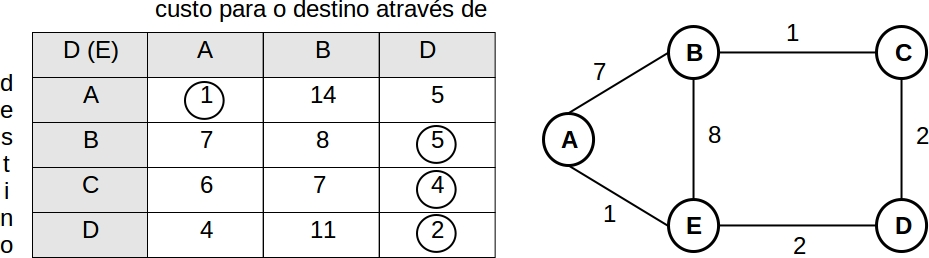
\includegraphics[scale=0.35]{vetor_de_distancia.jpg}
\end{figure}
\begin{itemize}
 \item A partir dos valores selecionados é criada a tabela de roteamento
 \item Periodicamente, cada roteador envia um cópia da sua tabela de roteamento aos roteadores adjacentes % quando ocorre mudanças na rede, stop() quando a ocorre mais troca de mensagem
\end{itemize}
\end{frame}

\begin{frame}{Mapas Métricos}
Periodicamente, cada roteador:
\begin{itemize}
 \olditem verifica o estado de seus enlaces % através do envio de pequenas mensagens
 \olditem envia as informações do estado dos enlaces aos roteadores adjacentes % quando ocorre mudanças na rede, stop() quando a ocorre mais troca de mensagem
\end{itemize}
\end{frame}

\begin{frame}{Mapas Topológicos}
Periodicamente, cada roteador:
\begin{itemize}
 \olditem verifica o estado de seus enlaces % através do envio de pequenas mensagens
 \olditem envia as informações do estado dos enlaces aos roteadores adjacentes % quando ocorre mudanças na rede, stop() quando a ocorre mais troca de mensagem
\end{itemize}
\end{frame}

\begin{frame}{SLAM}
\begin{itemize}
 \item O \textit{Open Shortest Path First} (OSPF) é um protocolo de roteamento interno % 
 \item Pertence a classe \textbf{estado de enlace} % 
 \item Utiliza o algoritmo de Dijkstra para calcular o caminho mínimo de uma origem para cada destino da rede %
\end{itemize}
\end{frame}

\section{Localização em Rede de Sensores sem Fio} % Descreva o NS-3

\begin{frame}{Introdução}
\begin{itemize}
 \item O \textit{Network Simulator 3} (NS-3) é um simulador de eventos discretos % 
 \item Voltado principalmente para simulação de redes de computadores %  
 \item É um software livre % 
 \item É construído como um sistema de bibliotecas escritas em C++ % 
\end{itemize}
\end{frame}

\begin{frame}{TOA(\textit{Time of Arrival})}
Os desafios de simular o OSPF já se iniciam na instalação
\begin{itemize}
 \item Três guias de instalação diferentes %  Uma para o somente o NS-3, uma para NS-3 + DCE, uma para NS-3 + DCE + Quagga
  \begin{enumerate}
   \olditem Somente o NS-3 % 
   \olditem O NS-3 e o DCE %
   \olditem O NS-3 e o DCE com suporte para o Quagga % 
  \end{enumerate}
  \begin{itemize}
   \olditem O DCE é um módulo do NS-3 que oferece suporte a aplicações reais % 
   \olditem O Quagga fornece implementações de protocolos de roteamento %
   \olditem O DCE e o Quagga são descritos com mais detalhes a seguir %
  \end{itemize}
 \item São necessários diversos pacotes % 
 \item Cada guia de instalação lista pacotes diferentes % 
 \item Alguns dos pacotes não são listados em nenhuma das guias % 
\end{itemize}
\end{frame}

\begin{frame}{TDOA(\textit{Time Difference of Arrival of Two Different Signals})}
Os desafios de simular o OSPF já se iniciam na instalação
\begin{itemize}
 \item Três guias de instalação diferentes %  Uma para o somente o NS-3, uma para NS-3 + DCE, uma para NS-3 + DCE + Quagga
  \begin{enumerate}
   \olditem Somente o NS-3 % 
   \olditem O NS-3 e o DCE %
   \olditem O NS-3 e o DCE com suporte para o Quagga % 
  \end{enumerate}
  \begin{itemize}
   \olditem O DCE é um módulo do NS-3 que oferece suporte a aplicações reais % 
   \olditem O Quagga fornece implementações de protocolos de roteamento %
   \olditem O DCE e o Quagga são descritos com mais detalhes a seguir %
  \end{itemize}
 \item São necessários diversos pacotes % 
 \item Cada guia de instalação lista pacotes diferentes % 
 \item Alguns dos pacotes não são listados em nenhuma das guias % 
\end{itemize}
\end{frame}


\begin{frame}{AOA(\textit{Angle of Arrival})}
Os desafios de simular o OSPF já se iniciam na instalação
\begin{itemize}
 \item Três guias de instalação diferentes %  Uma para o somente o NS-3, uma para NS-3 + DCE, uma para NS-3 + DCE + Quagga
  \begin{enumerate}
   \olditem Somente o NS-3 % 
   \olditem O NS-3 e o DCE %
   \olditem O NS-3 e o DCE com suporte para o Quagga % 
  \end{enumerate}
  \begin{itemize}
   \olditem O DCE é um módulo do NS-3 que oferece suporte a aplicações reais % 
   \olditem O Quagga fornece implementações de protocolos de roteamento %
   \olditem O DCE e o Quagga são descritos com mais detalhes a seguir %
  \end{itemize}
 \item São necessários diversos pacotes % 
 \item Cada guia de instalação lista pacotes diferentes % 
 \item Alguns dos pacotes não são listados em nenhuma das guias % 
\end{itemize}
\end{frame}

\begin{frame}{RSS(\textit{Received Signal Strength})}
Os desafios de simular o OSPF já se iniciam na instalação
\begin{itemize}
 \item Três guias de instalação diferentes %  Uma para o somente o NS-3, uma para NS-3 + DCE, uma para NS-3 + DCE + Quagga
  \begin{enumerate}
   \olditem Somente o NS-3 % 
   \olditem O NS-3 e o DCE %
   \olditem O NS-3 e o DCE com suporte para o Quagga % 
  \end{enumerate}
  \begin{itemize}
   \olditem O DCE é um módulo do NS-3 que oferece suporte a aplicações reais % 
   \olditem O Quagga fornece implementações de protocolos de roteamento %
   \olditem O DCE e o Quagga são descritos com mais detalhes a seguir %
  \end{itemize}
 \item São necessários diversos pacotes % 
 \item Cada guia de instalação lista pacotes diferentes % 
 \item Alguns dos pacotes não são listados em nenhuma das guias % 
\end{itemize}
\end{frame}


\section{Android} % Detalhe os experimentos que vc fez no NS-3
\begin{frame}{Introdução}
Criar uma simulação no NS-3 é relativamente simples
\begin{itemize}
 \item Documentação detalhada %  
 \item Diversos exemplos % 
 \item Diversos mecanismos de monitoramento, porém alguns deles exijem determinado nível de conhecimento % 
 \item Oferece alguns desafios como, por exemplo, a documentação sobre falhas de enlace é escassa % 
\end{itemize}
\end{frame}

\begin{frame}{Arquitetura}
\begin{itemize}
 \item Em simulações sem falhas o roteamento ocorre de acordo com o esperado %  
 \item Quando ocorre uma falha os pacotes que utilizam o caminho falho não chegam aos seus destinos % 
 \item Não é calculado um novo caminho mínimo % portanto
 \item Os roteadores não são informados sobre a falha do enlace % porque
  \begin{enumerate}
   \olditem Não é implementado o protocolo \textit{Hello} para identificar a falha % 
   \olditem Não é implementado o protocolo \textit{Flooding} para informar todos os roteadores %
  \end{enumerate}
 \item Somente o protocolo \textit{Exchange} está implementado no NS-3 % não é exatamente o exchange mas tem a mesma função
\end{itemize}
\end{frame}

\section{Componentes de uma Aplicação Android}
\begin{frame}{O Módulo DCE}
\begin{itemize}
 \item O NS-3 não fornece a implementação completa do OSPF % 
 \item O módulo \textit{Direct Code Execution} (DCE) passa a ser uma alternativa para simular o OSPF %  
 \item O DCE possui a implementação do protocolo OSPF feita pela \textit{Quagga Routing Suite} % 
 \item O DCE também permite utilizar executáveis do sistema operacional Linux % 
\end{itemize}
\end{frame}

\section{Implementação}
\begin{frame}{Conclusão}
\begin{itemize}
 \item Usar o DCE implica em trabalhar com a própria implementação do protocolo no sistema operacional % 
 \item Elimina a vantagem da simulação, na medida em que múltiplos detalhes devem ser considerados mesmo para testes simples %  
 \item É possível concluir que o trabalho futuro necessário, para permitir a continuidade deste trabalho, é completar a implementação do OSPF nativa do NS-3 % 
\end{itemize}
\end{frame}

\section{Conclusão}
\begin{frame}{Conclusão}
\begin{itemize}
 \item Usar o DCE implica em trabalhar com a própria implementação do protocolo no sistema operacional % 
 \item Elimina a vantagem da simulação, na medida em que múltiplos detalhes devem ser considerados mesmo para testes simples %  
 \item É possível concluir que o trabalho futuro necessário, para permitir a continuidade deste trabalho, é completar a implementação do OSPF nativa do NS-3 % 
\end{itemize}
\end{frame}

\end{document}
